\documentclass{article}
\usepackage[utf8]{inputenc}
\usepackage[T2A]{fontenc}
\usepackage{amsmath}
\usepackage{faktor} 
\usepackage{mathrsfs}
\usepackage[english,russian]{babel}
\usepackage{amssymb}
\usepackage{mathtools}
\usepackage{amsthm}
\usepackage{float}
\usepackage[shortlabels]{enumitem}
\usepackage[left=2cm,right=2cm, top=2cm,bottom=2cm,bindingoffset=0cm]{geometry}

\DeclareMathOperator{\ord}{ord}
\DeclareMathOperator{\orb}{Orb}
\DeclareMathOperator{\stab}{Stab}
\DeclareMathOperator{\lcm}{lcm}
\DeclareMathOperator{\inn}{Inn}
\DeclareMathOperator{\Ker}{Ker}
\DeclareMathOperator{\im}{Im}
\DeclareMathOperator{\tr}{tr}
\DeclareMathOperator{\rk}{rk}
\DeclareMathOperator{\interior}{int}
\DeclareMathOperator{\conv}{conv}
\DeclareMathOperator{\dom}{dom}
\DeclareMathOperator*{\argmax}{arg\,max}
\DeclareMathOperator{\diag}{diag}
\DeclareMathOperator{\cone}{cone}
\DeclareMathOperator{\sign}{sign}
\DeclareMathOperator{\rint}{rint}
\DeclareMathOperator{\aff}{aff}

\newcommand*{\QED}{\null\nobreak\hfill\ensuremath{\square}}
\newcommand*{\R}{\mathbb{R}}

\title{Subgradient and subdifferential}
\author{Ковалев Алексей}
\date{}

\begin{document}

\maketitle

\paragraph{1.}
\[ f(x) = \text{PReLU}(x) = \begin{cases}
    x, & x > 0 \\
    ax, & x \leqslant 0
\end{cases} \]
По определению $ g \in \partial f(x_0) \iff \forall x \in \dom f $ выполняется неравенство $ f(x) \geqslant f(x_0) + \langle g,\, x - x_0 \rangle $.
\begin{itemize}
    \item Пусть $a > 1$. Ясно, что при этом функция не выпукла. В точке $x_0 \neq 0$ функция дифференцируема, а значит $\partial f(x_0) = \varnothing$ или $\partial f(x_0) = \{ \nabla f(x_0) \}$. Но при этом по критерию выпуклости $\forall x \in \dom f$ выполняется $f(x) < f(x_0) + \langle \nabla f(x_0),\, x - x_0 \rangle$, то есть $\nabla f(x_0) \not \in \partial f(x_0)$ при $x_0 \neq 0$.
        При $x_0 = 0$ получаем $g \in \partial f(x_0) \iff \forall x \in \dom f$ выполняется $f(x) \geqslant gx$, а значит $x \geqslant gx,\, x > 0$ и $ax \geqslant gx,\, x \leqslant 0$. То есть $1 \geqslant g \geqslant a > 1$. Значит $\partial f(x) = \varnothing$ при любом $x$.
    \item Пусть $a \leqslant 1$. Тогда функция выпукла и из критерия выпуклости и теоремы о субдифференциале дифференцируемой функции получаем $\partial f(x_0) = \{ \nabla f(x_0) \}$ при $x_0 \neq 0$.
        При $x_0$ получаем $g \in \partial f(x_0) \iff \forall x \in \dom f$ выполняется $f(x) \geqslant gx$, а значит $x \geqslant gx,\, x > 0$ и $ax \geqslant gx,\, x \leqslant 0$. То есть $1 \geqslant g \geqslant a$.
\end{itemize}
\textbf{Ответ:} $\partial f(x) = \varnothing$ при $a > 1$ и $\partial f(x) = \begin{cases} 1, & x > 0 \\ [a; 1], & x = 0 \\ a, & x < 0 \end{cases}$ при $a \leqslant 1$.


\paragraph{2.} $0 \in \partial f(x_0) \iff \forall x \in \dom f$ выполняется неравенство $f(x) \geqslant f(x_0) + \langle 0,\, x - x_0 \rangle = f(x_0) \iff x_0$ -- точка минимума функции $f$. \QED 


\paragraph{3.} $f(x) = \| Ax - b \|_1$. Пусть $\varphi(x) = Ax - b$. Тогда $f = \| \cdot \|_1 \circ \varphi$. \\
В таком случае субдифференциал $\partial f(x) = \partial(\| \cdot \|_1 \circ \varphi)(x) = A^{\top} \partial \| \cdot \|_1(\varphi(x)) = A^{\top} \partial \| \cdot \|_1 (Ax - b)$. При этом
\[ \partial \| \cdot \|_1 (x) = \begin{cases}
    B_{\| \cdot \|_\infty}(0,\, 1), & x = 0 \\
    \left\{ s :\: s \in \R^n,\, \| s \|_\infty = 1,\, \langle s,\, x \rangle = \| x \|_1 \right\}, & x \neq 0 
\end{cases} \]
\textbf{Ответ:} $\partial f(x) = \begin{cases}
    \left\{ A^\top s :\: s \in B_{\| \cdot \|_\infty}(0,\, 1) \right\}, & Ax - b = 0 \\
    \left\{ A^\top s :\: s \in \R^n,\, \| s \|_\infty = 1,\, \langle s,\, Ax - b \rangle = \| Ax - b \|_1 \right\}, & Ax - b \neq 0 
\end{cases}$ 


\paragraph{4.} $f(x) = e^{\| x \|}$. $e^x$ -- выпуклая, монотонно неубывающая, дифференцируемая функция, $\| \cdot \|$ -- выпуклая функция, а значит справедлива формула для субдифференциала сложной функции \\
\[ \partial f(x) = \partial e^{\| \cdot \|}(x) = e^{\| x \|} \partial \| \cdot \|(x) \]
Воспользуемся формулой для субдифференциала нормы
\[ \partial \| \cdot \| (x) = \begin{cases}
    B_{\| \cdot \|_\ast}(0,\, 1), & x = 0 \\
    \left\{ s :\: s \in \R^n,\, \| s \|_\ast = 1,\, \langle s,\, x \rangle = \| x \| \right\}, & x \neq 0 
\end{cases} \]
\textbf{Ответ:} $\partial f(x) = \begin{cases}
    B_{\| \cdot \|_\ast}(0,\, 1), & x = 0 \\
    \left\{ e^{\| x \|} s :\: s \in \R^n,\, \| s \|_\ast = 1,\, \langle s,\, x \rangle = \| x \| \right\}, & x \neq 0 
\end{cases}$ 


\paragraph{5.} $f(x) = \frac12 \| Ax - b \|_2^2 + \lambda \| x \|_1$, где $\lambda > 0$. \\
Сначала найдем $\partial g(x)$, где $g(x) = \frac12 \| Ax - b \|_2$ аналогично номеру 3.
\[ \partial g(x) = \begin{cases}
    \left\{ A^\top s :\: s \in B_{\| \cdot \|_2}(0,\, 1) \right\}, & Ax - b = 0 \\
    \left\{ A^\top s :\: s \in \R^n,\, \| s \|_2 = 1,\, \langle s,\, Ax - b \rangle = \| Ax - b \|_2 \right\}, & Ax - b \neq 0 
\end{cases} \]
Теперь воспользуемся формулой для субдифференциала сложной функции для $h(x) = \| Ax - b \|_2^2$. Эта формула справедлива, так как $x^2$ -- выпуклая, монотонно неубывающая, дифференцируемая на $\R_+$ функция, $\| Ax - b \|_2$ -- выпуклая функция.
\[ \partial h(x) = \| Ax - b \|_2 \partial g(x) \]
Наконец, пользуясь теоремой Моро-Рокафеллара, получем
\[ \begin{aligned}
    \partial f(x) \\
    &= \partial h(x) + \lambda \partial \| \cdot \|_1 (x) \\ 
    &= \begin{cases}    
        \left\{ 0 \right\}, & Ax - b = 0 \\
        \left\{ \| Ax - b \|_2 \cdot A^\top s :\: s \in \R^n,\, \| s \|_2 = 1,\, \langle s,\, Ax - b \rangle = \| Ax - b \|_2 \right\}, & Ax - b \neq 0 
    \end{cases} \\ 
    &+ \begin{cases}
        B_{\| \cdot \|_\infty}(0, \lambda), & x = 0 \\
        \left\{ \lambda s :\: s \in \R^n,\, \|s\|_\infty = 1,\, \langle s,\, x \rangle = \|x\|_1 \right\}, & x \neq 0
    \end{cases}
\end{aligned} \]
\textbf{Ответ:} приведен выше.


\paragraph{6.} $N_S(x) = \{ c :\: c \in \R^n,\, \forall y \in S \; \langle c,\, y - x \rangle \leqslant 0 \}$ -- нормальный конус множества $S$ в точке $x$.
\begin{enumerate}[(a)]
    \item Нормальные конусы на самом деле находятся в точке 0, но для удобства каждый конус смещен смещены в точку, к которой он относится. Конусы построены из тех соображений, что вектор лежит в нем тогда и только тогда, когда он образует угол $\geqslant 90^\circ$ с любым вектором множества.
        \begin{figure}[H]
            \centering
            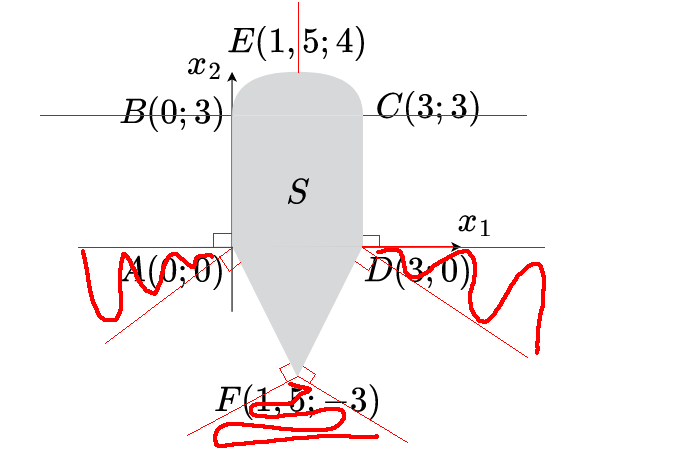
\includegraphics[scale=0.4]{nakovalnya_rusov.png}
        \end{figure}
    \item Пусть $x \in \rint S$. Пусть также $0 \neq c \in N_S(x) = \{ c :\: c \in \R^n,\, \forall y \in S \; \langle c,\, y - x \rangle \leqslant 0 \}$. Ясно, что в $\rint S$ найдутся $x_1,\, x_2$, такие что $x - x_1 = x_2 - x$, так как $x \in \rint S \iff x \in U(x) \cap \aff S$, где $U(x)$ -- какая-то окрестность $x$. Тогда $\langle c,\, x - x_1 \rangle \leqslant 0$ и $\langle c,\, x_2 - x \rangle \geqslant 0$. Но $x - x_1 = x_2 - x$, а значит $\langle c,\, x - x_1 \rangle = 0$ и $c = 0$. \QED
        % Это неверно. Контрпример -- отрезок на оси $x$ на плоскости. Тогда любой вектор перпендикулярный оси $x$ лежит в $N_S(x)$.
    \item  
        \[ I_S(x) = \begin{cases}
            0, & x \in S \\ 
            \infty, & x \not \in S
        \end{cases} \]
        Требуется показать, что $\partial I_S(x) = N_S(x)$, но это справедливо только для точек $x \in S$. Пусть $x_0 \in S$.
        \[ \partial I_S(x_0) = \{ g :\: \forall x \in \R^2 \; I_S(x) \geqslant I_S(x_0) + \langle g,\, x - x_0 \rangle \} = \{ g :\: \forall x \in S \; 0 \geqslant \langle g,\, x - x_0 \rangle \} = N_S(x_0) \]
        Пусть теперь $x_0 \not \in S$. Тогда $N_S(x_0) = \{ 0 \}$, в то время как
        \[ \partial I_S(x_0) = \{ g :\: \forall x \in \R^2 \; I_S(x) \geqslant I_S(x_0) + \langle g,\, x - x_0 \rangle \} = \{ g :\: \forall x \in \R^2 \; I_S(x) \geqslant \infty + \langle g,\, x - x_0 \rangle \} = \varnothing \]
        Значит для любого $x \in S$ $\partial I_S(x) = N_S(x)$, а для любого $x \not \in S$ $\partial I_S(x) \neq N_S(X)$.
\end{enumerate}


\end{document}
